\documentclass{bmcart}

%%%%%%%%%%%%%%%%%%%%%%%%%%%%%%%%%%%%%%%%%%%%%%
%%                                          %%
%% CARGA DE PAQUETES DE LATEX               %%
%%                                          %%
%%%%%%%%%%%%%%%%%%%%%%%%%%%%%%%%%%%%%%%%%%%%%%

%%% Load packages
\usepackage{amsthm,amsmath}
\usepackage{graphicx}
%\RequirePackage[numbers]{natbib}
%\RequirePackage{hyperref}
\usepackage[utf8]{inputenc} %unicode support
%\usepackage[applemac]{inputenc} %applemac support if unicode package fails
%\usepackage[latin1]{inputenc} %UNIX support if unicode package fails


%%%%%%%%%%%%%%%%%%%%%%%%%%%%%%%%%%%%%%%%%%%%%%
%%                                          %%
%% COMIENZO DEL DOCUMENTO                   %%
%%                                          %%
%%%%%%%%%%%%%%%%%%%%%%%%%%%%%%%%%%%%%%%%%%%%%%

\begin{document}

	\begin{frontmatter}
	
		\begin{fmbox}
			\dochead{Research}
			
			%%%%%%%%%%%%%%%%%%%%%%%%%%%%%%%%%%%%%%%%%%%%%%
			%% INTRODUCIR TITULO PROYECTO               %%
			%%%%%%%%%%%%%%%%%%%%%%%%%%%%%%%%%%%%%%%%%%%%%%
			
			\title{Implicación del gen de la subunidad beta-3 de la proteína G en la diabetes materna}
			
			%%%%%%%%%%%%%%%%%%%%%%%%%%%%%%%%%%%%%%%%%%%%%%
			%% AUTORES. METER UNA ENTRADA AUTHOR        %%
			%% POR PERSONA                              %%
			%%%%%%%%%%%%%%%%%%%%%%%%%%%%%%%%%%%%%%%%%%%%%%
			
			\author[
			  addressref={aff1},                   % ESTA LINEA SE COPIA IGUAL PARA CADA AUTOR
			  corref={aff1},                       % ESTA LINEA SOLO DEBE TENERLA EL COORDINADOR DEL GRUPO
			  email={victorgo@uma.es}   % VUESTRO CORREO ACTIVO
			]{\inits{V.G.O}\fnm{Víctor} \snm{Guirado Osorio}} % inits: INICIALES DE AUTOR, fnm: NOMBRE DE AUTOR, snm: APELLIDOS DE AUTOR
			\author[
			  addressref={aff2},
			  email={susanafernandez@uma.es}
			]{\inits{S.R.F.G}\fnm{Susana R.} \snm{Fernández Giaccomassi}}
			\author[
			addressref={aff3},
			email={pablobermudezgamez@uma.es}
			]{\inits{P.B.G}\fnm{Pablo} \snm{Bermúdez Gámez}}
			\author[
			addressref={aff4},
			email={juancavergara6@uma.es}
			]{\inits{J.C.V.R}\fnm{Juan C.} \snm{Vergara Ruz}}
			
			%%%%%%%%%%%%%%%%%%%%%%%%%%%%%%%%%%%%%%%%%%%%%%
			%% AFILIACION. NO TOCAR                     %%
			%%%%%%%%%%%%%%%%%%%%%%%%%%%%%%%%%%%%%%%%%%%%%%
			
			\address[id=aff1]{%                           % unique id
			  \orgdiv{ETSI Informática},             % department, if any
			  \orgname{Universidad de Málaga},          % university, etc
			  \city{Málaga},                              % city
			  \cny{España}                                    % country
			}
		
		\end{fmbox}% comment this for two column layout
		
		\begin{abstractbox}
		
			\begin{abstract} % abstract
			
			
			Durante el embarazo, diversos mecanismos fisiológicos se ven afectados, incluyendo la regulación de leptina, adiponectina y la gluconeogénesis, lo que puede desencadenar complicaciones relacionadas con la diabetes materna (DM). Un mecanismo biológico de particular interés es la posible relación entre la DM y la subunidad beta-3 de la proteína G (GNB3), que está implicado en la ganancia de peso y la obesidad, factores que son conocidos por incrementar la resistencia a la insulina. Nuestro estudió reveló la contribución del gen GNB3 en la DM, profundizando en su papel en la regulación de la glucosa.
			
			
			\end{abstract}
			
			%%%%%%%%%%%%%%%%%%%%%%%%%%%%%%%%%%%%%%%%%%%%%%
			%% PALABRAS CLAVE DEL PROYECTO              %%
			%%%%%%%%%%%%%%%%%%%%%%%%%%%%%%%%%%%%%%%%%%%%%%
			
			\begin{keyword}
			\kwd{diabetes materna}
			\kwd{insulina}
			\kwd{GNB3}
			\end{keyword}
		
		
		\end{abstractbox}
	
	\end{frontmatter}
	
	
	%%%%%%%%%%%%%%%%%%%%%%%%%%%%%%%%%
	%% COMIENZO DEL DOCUMENTO REAL %%
	%%%%%%%%%%%%%%%%%%%%%%%%%%%%%%%%%
	
	\section{Introducción}
Se estima que el gasto en salud en personas diabéticas a nivel mundial en 2017 fue de 850 mil millones de dólares \cite{Cho2018} y que las mujeres que padecen diabetes durante la gestación tienen diez veces más riesgo de desarrollar diabetes mellitus tipo 2 (DMT2) que mujeres con un embarazo normal \cite{Vounzoulaki2020} \cite{You2021}. La prevalencia de hiperglucemia en el embarazo entre mujeres de 20 a 49 años es de un 16% y la cifra va en aumento \cite{Guariguata2014}.

Se asocia a la DM con enfermedades cardiacas en el feto \cite{Depla2021} e incluso con enfermedades cardiovasculares y cerebrovasculares en la madre \cite{Xie2022}.

	\section{Materiales y métodos}

\subsection{Materiales}
Los genes relacionados con el fenotipo ``Maternal diabetes'' (HP:0009800) fueron extraídos de la base de datos Human Phenotype Ontology (HPO) en la web hpo.jax \cite{Kohler2017}. Específicamente, se trabajó con una lista de 43 genes asociados al fenotipo, la cual se encontraba en formato excel.

Se utilizaron las librerías de Python
%La API de StringDB \cite{Szklarczyk2015} como la herramienta principal.
openpyxl 3.1.2, Stringdb 0.1.5 \cite{Mering2005}, Pandas 2.1.2 \cite{McKinney2015}, iGraph 0.11.2 \cite{Csardi2006} y Cairocffi 1.6.1, para el procesamiento de datos y las representaciones.

%La configuración e instalación necesarias se llevaron a cabo mediante scripts en Bash \cite{Dong2023}.

Ejecutado en un MacBook Air 15 con Intel Core i5-5250U CPU 1.60GHz, 8 GB RAM y sistema operativo Ubuntu 22.04.3 LTS (Jammy Jellyfish).

\subsection{Metodología}

EL flujo de trabajo que se siguió puede observarse en la figura \ref{fig:workflow} y que se explicará en detalle a continuación.

\begin{figure}[h!]
	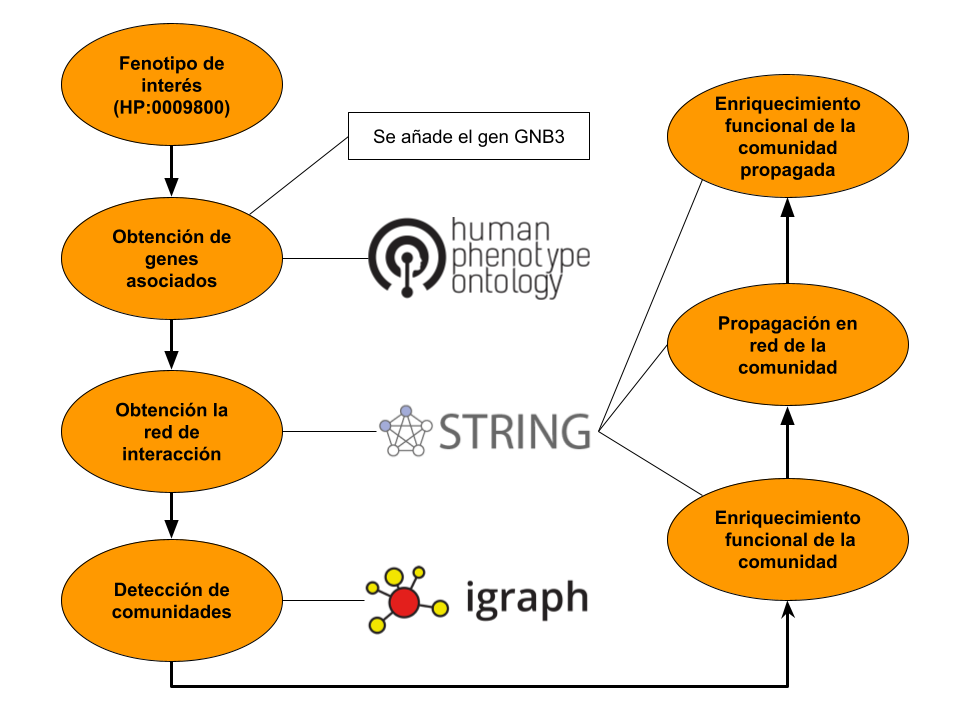
\includegraphics[width=0.9\textwidth]{figures/workflow.png}
	\caption{Flujo de trabajo: Se representa el flujo de trabajo seguido para la realización del proyecto. Empieza desde la obtención de los genes asociados al fenotipo de interés y la creación de la red de interacción hasta el análisis por enriquecimiento funcional.}
	\label{fig:workflow}
\end{figure}

Descargamos la lista de genes implicados al fenotipo HP:0009800 directamente desde HPO en formato excel e insertamos en la lista el gen GNB3.

Utilizamos la librería stringdb de Python para obtener la red de interacción de los genes asociados al fenotipo.

Mediante la librería de igraph se construyó la red de interacción de genes y se realizó un algoritmo de detección de comunidades basado en ``edge betweenness'' \cite{Girvan2002}. Una vez realizada la detección, se seleccionó la comunidad donde estaba presente el gen GNB3.

Realizamos un enriquecimiento funcional de los genes que formaban parte de esa comunidad con la librería de stringdb. 

Se creó una nueva red mediante una propagación en red de los genes presentes en la comunidad de interés con un nuevo parámetro de entrada para añadir 16 genes más. A partir de esta red volvimos a realizar un enriquecimiento funcional.

	
\section{Resultados}

\subsection{Visión General}

Hemos investigado el uso de la biología de sistemas para entender mejor el fenotipo diabetes materna. En esta sección presentaremos los resultados del análisis de la red de genes relacionados con el fenotipo a partir de datos de interacción proteína-proteína descargados de STRINGdb con el propósito de estudiar la relación entre la diabetes materna y el gen GNB3.

A continuación procederemos a detallar los resultados obtenidos al ejecutar nuestro flujo de trabajo.

\subsection{Red de interacción}

Al acceder a la base de datos HPO observamos que la cantidad de enfermedades asociadas a la DM es 31, y al descargar la lista de genes implicados en el fenotipo de estudio, vemos que el número de genes asociados es de 43. Hemos generado la red de interacción entre estos genes para obtener la cantidad de nodos e interacciones entre ellos. En la Tabla~\ref{table:nodes_edges_count} se puede observar la cantidad de nodos (genes) y edges (interacciones) de la red sin incluir el gen GNB3 e incluyendo al gen para hacer la red.


\begin{table}[h]
	\centering
	\caption{Cantidad de nodos e interacciones: Se ha creado la red de interacciones de los genes relacionados con el fenotipo y otra red añadiendo al gen de estudio. Finalmente, se ha obtenido la cantidad de nodos y edges de cada red.}
	\label{table:nodes_edges_count}
	\begin{tabular}{|c|c|c|}
		\hline
		\textbf{Red} & \textbf{Nodos} & \textbf{Edges} \\ \hline
		Sin GNB3 & 43    & 272   \\ \hline
		Con GNB3 & 44    & 276  \\ \hline
	\end{tabular}

\end{table}

La red generada por stringdb usando los genes asociados a la diabetes materna y el GNB3 se pude observar en la Figura~\ref{fig:network}.

\begin{figure}[h!]
	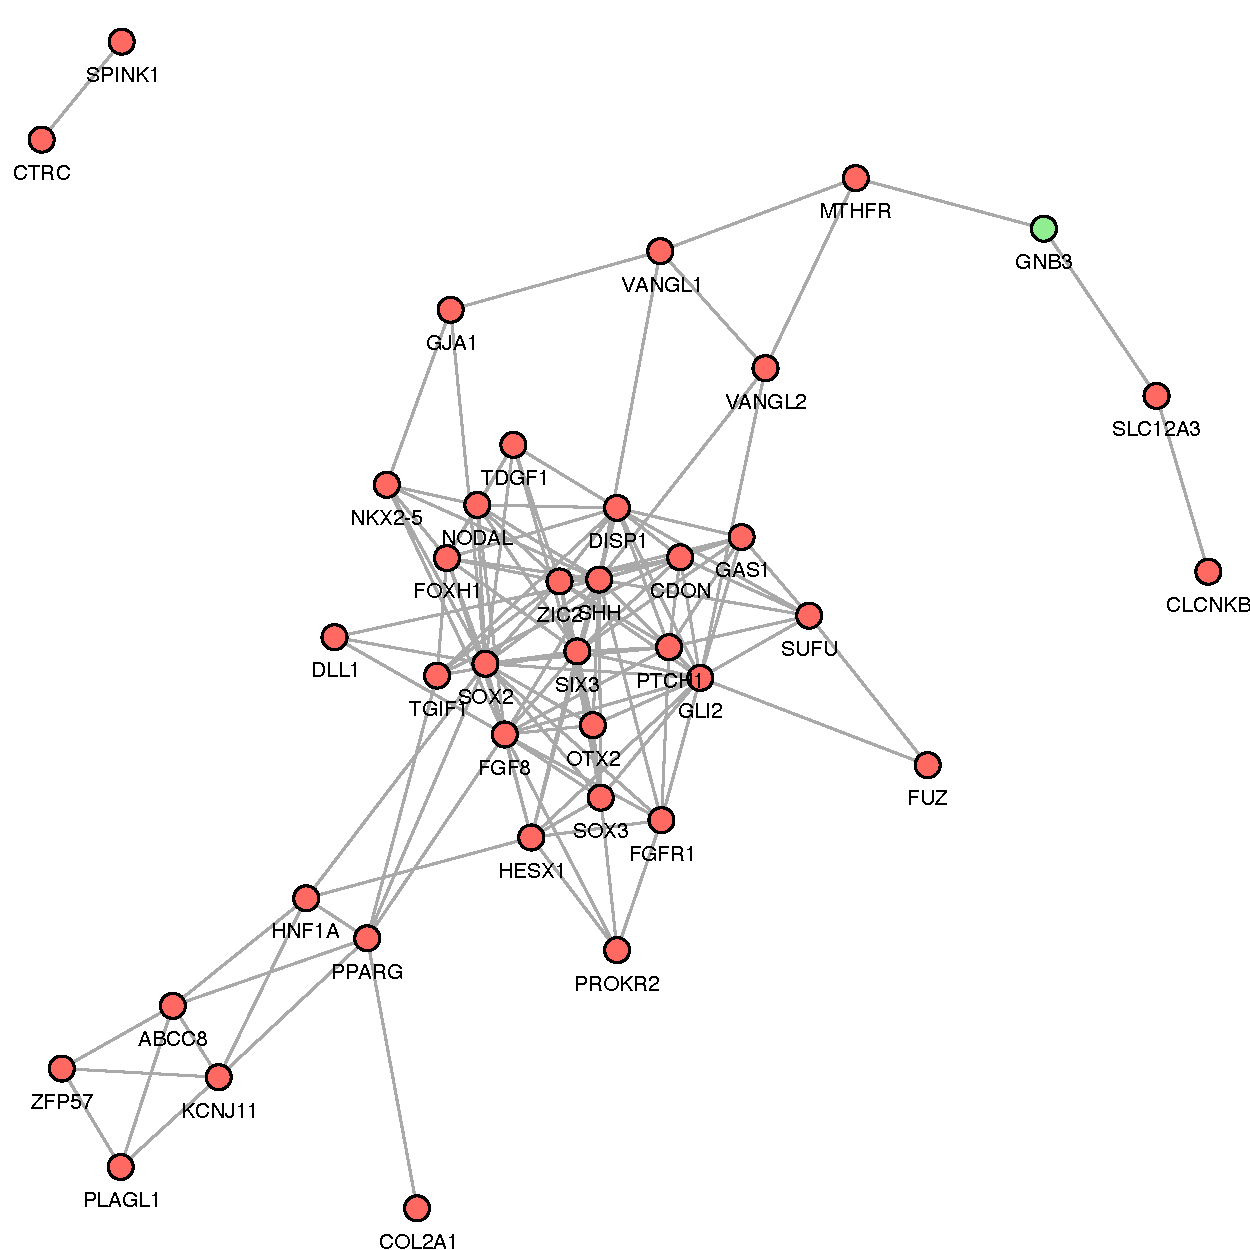
\includegraphics[width=0.9\textwidth]{figures/network.pdf}
	\caption{Red de Interacción: Se observan las interacciones entre los genes asociados al fenotipo de estudio y el gen GNB3. Los nodos en rojo representan los genes asociados al fenotipo, mientras que el nodo verde representa al GNB3.}
	\label{fig:network}
\end{figure}

\subsection{Detección de comunidades}

Hemos detectado las comunidades de la red obtenida en el paso anterior, usando el método ``edge betweenness'' descrito en la sección de métodos. Obtuvimos cinco comunidades a partir de la red de interacciones. El GNB3 se encuentra presente en una comunidad con otros dos nodos, los genes SLC12A3 y el CLCNKB, como puede observarse en la Figura~\ref{fig:comunidad}.

\begin{figure}[h!]
	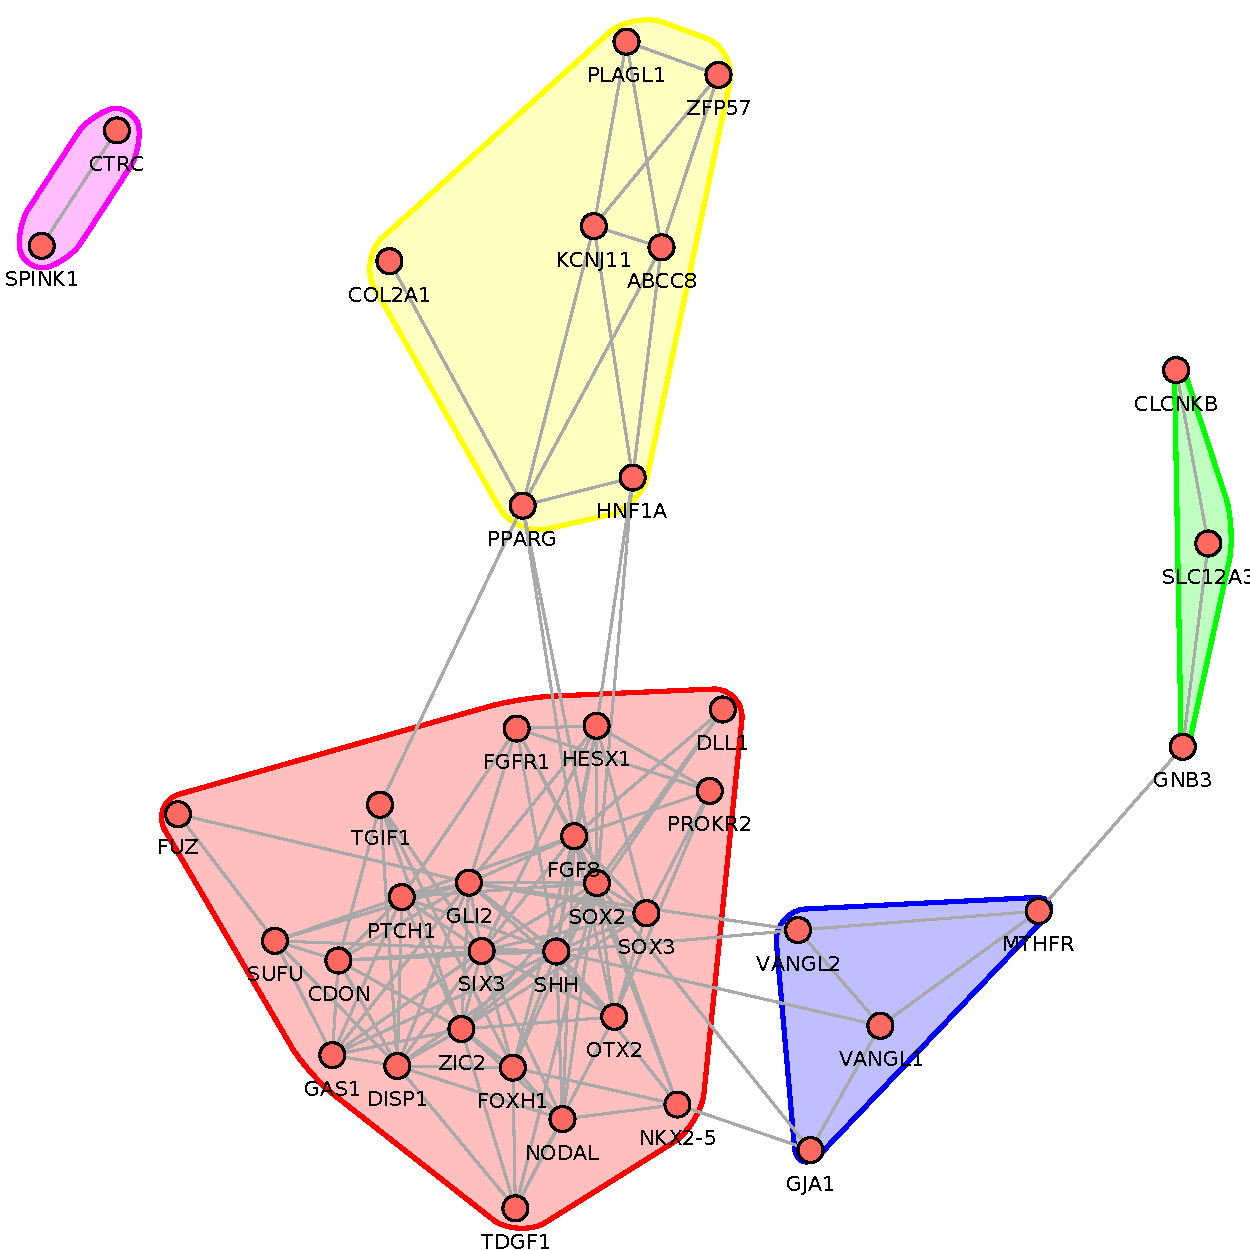
\includegraphics[width=0.9\textwidth]{figures/comunidades.pdf}
	\caption{Detección de comunidades: Se representa la clusterización de los nodos en cinco comunidades.}
	\label{fig:comunidad}
\end{figure}

\subsection{Enriquecimiento funcional}

Una vez detectada la comunidad a la que pertenece el gen GNB3 en la red de estudio, hemos obtenido el enriquecimiento funcional para los tres genes pertenecientes a la comunidad.  Filtrando aquellos resultados en los que aparece el gen GNB3, el análisis demostró un enriquecimiento para el fenotipo HPO de anormalidad de la visión, con un p-valor de 0.00021, como se puede observar en la Tabla~\ref{table:enriquecimiento1}

\begin{table}[h]
	\centering
	\caption{Enriquecimiento funcional de la comunidad del gen GB3: Se observa el único resultado para el gen de interés.}
	\label{table:enriquecimiento1}
	\begin{tabular}{|c|c|c|c|c|c|}
		\hline
		\textbf{Preferred Names} & \textbf{Description} & \textbf{P-value} & \textbf{fdr} & \textbf{Category} & \textbf{Term} \\ \hline
		GNB3, CLCNKB, SLC12A3 & Abnormality of vision    & 0.00021 & 0.0197&  HPO & HP:0000504 \\ \hline

	\end{tabular}

\end{table}

\subsection{Propagación de la red}

Hemos realizado la propagación de la red añadiendo 16 nodos más, que interaccionan con los tres genes pertenecientes a la comunidad del gen GNB3. A continuación, hemos procedido a realizar el enriquecimiento funcional incluyendo los nuevos genes. En este caso, el gen de interés apareció implicado en 96 procesos, de los cuales se muestran aquellos relacionados con la regulación de insulina y glucagón en la Tabla~\ref{table:enriquecimiento2}. Se puede observar que, en todos los casos representados, hay un enriquecimiento significativo en términos relacionados con RCTM, que ha sido introducido en la sección de métodos.


\begin{table}[h]
	\centering
	\caption{Enriquecimiento funcional de la comunidad del gen GB3 expandida: Se observan los resultados que incluyen al gen GNB3 y que incluyen mecanismos relacionados con la insulina o el glucagón. Todos los resultados son de la categoría RCTM.}
	\label{table:enriquecimiento2}
	\begin{tabular}{|c|c|c|c|}
		\hline
		 \textbf{Description} & \textbf{P-value} &\textbf{ fdr }&  \textbf{Term} \\ \hline
		 \begin{flushleft} Regulation of insulin secretion \end{flushleft} & 9.38e-30 & 1.05e-27 &   HSA-422356 \\ \hline
		 \begin{flushleft} Glucagon-like Peptide-1 (GLP1) regulates insulin secretion \end{flushleft} & 3.57e-30 & 5.44e-28  & HSA-381676 \\ \hline
		 \begin{flushleft} Adrenaline,noradrenaline inhibits insulin secretion \end{flushleft} & 3.88e-29 & 3.28e-27  & HSA-400042 \\ \hline
		 \begin{flushleft} Glucagon-type ligand receptors \end{flushleft} & 2.51e-31 & 5.73e-29  & HSA-420092 \\ \hline
		 \begin{flushleft} Glucagon-like Peptide-1 (GLP1) regulates insulin secretion \end{flushleft} & 3.57e-30 & 5.44e-28  & HSA-381676 \\ \hline
		 \begin{flushleft} Glucagon signaling in metabolic regulation \end{flushleft} & 1.31e-25 & 6.95e-24  & HSA-163359 \\ \hline
		 \begin{flushleft} Synthesis, secretion, and inactivation of Glucagon-like Peptide-1 (GLP-1) \end{flushleft} & 1.33e-06 & 4.39e-05  & HSA-381771 \\ \hline
	\end{tabular}

\end{table}

Después de haber presentado los resultados, la discusión de los mismos seguirá en la próxima sección.

	\section{Discusión}
Hemos encontrado que los genes implicados en el fenotipo de diabetes materna interactuaban con el gen GNB3 en mecanismos de regulación de insulina y glucagón. Lo cual está relacionado con problemas de obesidad que pueden afectar a pacientes con este fenotipo. Además, encontramos que un subconjunto de genes del fenotipo estaban implicados en una abnormalidad en la visión.

Ya se sospechaba que este gen estaba relacionado con la diabetes materna \cite{Feng2019} ya que ambos están implicados en procesos de regulación de insulina \cite{Rodolaki2023, Feng2019} que pueden producir problemas como la obesidad \cite{Shah2011}. También, un proceso alterado por la diabetes materna es la visión \cite{Nelson1986}, lo que pudimos observar en los resultados. Como se sospechaba hemos encontrado una relación entre la diabetes materna y el gen GNB3 en mecanismo implicados en la obesidad.

Nuestros resultados tiene una buena fuerza estadística ya que todos los procesos que hemos obtenido al hacer el enriquecimiento funcional presentan un p valor y un FDR bajos. También, hemos simplificado la rede formada para que solo exista una relación entre los nodos. Esto hace que la búsqueda de comunidades sea mucho más eficiente ya que solo nos interesa si un nodo está relacionado con otro, no si existe más de una evidencia que lo justifica.

Una limitación que presenta el estudio es que como no se obtuvieron procesos relacionados con la insulina en el primer enriquecimiento funcional, se realizó una propagación de la comunidad. Esto es un procedimiento correcto ya busca más nodos relacionados con la comunidad de estudio para encontrar más información. Sin embargo, este proceso realizado ha sido en parte buscado, es decir, para poder obtener dichos resultados ha sido necesario obtener los primeros resultados.


	\section{Conclusiones}

En conclusión, nuestros hallazgos respaldan la asociación entre los genes relacionados con la diabetes materna y el gen GNB3 mediante procesos de regulación metabólica. La fuerza estadística de nuestros resultados, respaldada por análisis de enriquecimiento funcional significativos, subraya la validez de nuestras observaciones. Esta investigación sienta las bases para futuras exploraciones tanto a nivel experimental como clínico.

Reiteramos la importancia de considerar los resultados en el contexto de posibles aplicaciones terapéuticas y destacamos la relevancia de la gestión de la diabetes materna para abordar problemas metabólicos durante el embarazo. En última instancia, nuestros hallazgos proporcionan conocimientos clave para la comprensión y manejo de las complejas interrelaciones genéticas subyacentes a la diabetes materna y sus implicaciones en la salud.


	
	
	%%%%%%%%%%%%%%%%%%%%%%%%%%%%%%%%%%%%%%%%%%%%%%
	%% OTRA INFORMACIÓN                         %%
	%%%%%%%%%%%%%%%%%%%%%%%%%%%%%%%%%%%%%%%%%%%%%%
	
	\begin{backmatter}
	
		\section*{Abreviaciones}%% if any
		DM: diabetes materna
		DMT2: diabetes mellitus tipo 2
		SNP: single nucleotide polymorphism 
		RCTM: Reactome
		FDR: tasa de descubrimiento falso
		
		\section*{Disponibilidad de datos y materiales}%% if any
			%https://github.com/ElArquitectorgo/systems_biology.git
		
		\section*{Contribución de los autores}
			V.G.O : redacción, revisión, código; S.R.F.G : introducción; P.B.G : redacción de la introducción, creación de una plantilla del workflow y del script para conseguir la red de genes de StringDB, redacción de la metodología y redacción de una parte de la discusión; J.C.V.R : introducción
		
		
		%%%%%%%%%%%%%%%%%%%%%%%%%%%%%%%%%%%%%%%%%%%%%%%%%%%%%%%%%%%%%%%%%%%%%%%%%%%%%%%%%%%%%%%%
		%% BIBLIOGRAFIA: no teneis que tocar nada, solo sustituir el archivo bibliography.bib %%
		%% por el que hayais generado vosotros                                                %%
		%%%%%%%%%%%%%%%%%%%%%%%%%%%%%%%%%%%%%%%%%%%%%%%%%%%%%%%%%%%%%%%%%%%%%%%%%%%%%%%%%%%%%%%%
		
		\bibliographystyle{bmc-mathphys} % Style BST file (bmc-mathphys, vancouver, spbasic).
		\bibliography{bibliography}      % Bibliography file (usually '*.bib' )
	
	\end{backmatter}
\end{document}
